\chapter{Solving the De Novo Genome Assembly}


In this last chapter we approach the genome assembly problem with the using quantum annealing. Let us first understand what this problem is. We will then translate it to a QUBO model and solve it using quanutm annealing.


\section{The Genome Assembly Problem}


The genome of an organism is all its genetic material \cite{Roth2019}. The deoxyribonucleic acid (DNA) is the carrier of that genetic information. It consists of two long chains twisted to form a double helix \cite{Alberts2007}. Each of these chains is composed of a series of nucleotides or bases: adenine (A), guanine (G), cytosine (C), and thymine (T). Since these bases are matched in pairs in the DNA double helix, those are called base pairs (bp).

A genome sequence is the complete list of nucleotides of every chromosome of an organism. With today's technology, automated sequence machines can read up to 1000 bp at a time \cite{Slatko2011} while the human genome contains 3 Mbp, so we cannot simply read the whole genome. This is where genome assembly comes in.

Genome assembly refers to the process of, given a large number of short DNA reads, stitch them together to form a large representation of the original chromosome where the reads came from. The two main techniques used to reconstruct these sequences are the ab initio reference-free alignment and the de novo reference-based assembly.


\subsection{Ab initio reference-based alignment}


In this method, the DNA reads are matched against a known trusted reference of the same organism. This is essentially a pattern matching problem, where we find the index of a given sub-string in a larger string. However, after the reconstruction is complete the result is compared to the reference in order to identify implications; therefore introducing bias based on the reference \cite{Sarkar2020}.

In the naive approach, the short sub-string is compared to the reference starting at the first index. If the end of the sub-string is reached with a positive, a match is obtained. Otherwise, the sub-string is shifted a single position and we compare again. Heuristic methods that improve on this idea are based on shifting a greater number of spaces after a mismatch.

Different number of strategies have been developed in this direction. For instance, the classic Boyer-Moore and Knuth-Pratt-Morris algorithms \cite{Holmes1999}. However, these in particular are not adequate for genome assembly since these are exact string matching algorithms and DNA reads usually need approximate matches due to reads errors. Other algorithms worth mentioning are the Needleman-Wunsch algorithm \cite{Needleman1970} and the Smith-Waterman algorithm \cite{Smith1981}, for global and local alignment respectively. These are dynamic programming algorithms designed specifically with DNA reads in mind. 

State of the art algorithms trades off accuracy for speed and memory. The approximation and errors introduced prevents the application of this technique to critical areas such as personalized medicine. Given enough computational power, the de novo method yields better results.


\subsection{De novo reference-free assembly}


On the other hand, the de novo reference-free method is, as its name suggests, reference free. Meaning, it is based only on the DNA reads. Thus, it has no reference bias but it is more computationally complex. It is usually used the first time a species DNA is read.

In this technique, multiple copies of the same DNA are made before slicing it. After chopping each copy at random places the data is redundant and the different reads overlap, making the assembly easier. There are multiple methods for de novo assembly based on different tools: Overlap-Layout Consensus (OLC) methods, de Bruijn graph (DBG) methods, string graphs, greedy and hybrid methods are some of the most famous examples. Depending on the reading method and the number and length of the DNA reads, different methods excel from the rest. For instance, short-read technologies with a large number of reads favor DBG methods while high-quality long reads favor OCL methods. For our purposes, we will focus on the OCL method.

In the OLC graph used for the de novo whole-genome assembly, each node represents a different DNA read. Directed edges are associated a weight depending on how well these two reads are stitched together in a certain order. For example, the directed edge going from reading $r_1$ to read $r_2$ will be assigned a weight depending on how well $r_1r_2$ can be stiched.

The weights computation depends on the implementation. For our purposes, we will use exact matches, no taking reading errors into consideration. Then, the weight assigned to an edge is the length of the overlap between both reads without any errors, with a change of sign. For example, given the reads $r_1 = AATT$ and $r_2 = TTCC$, the perfect stitching will produce $AATTCC$, so the overlap between both reads is $2$, giving a weight of $-2$. We may call this the \emph{distance} between reads $r_1$ and $r_2$ (in that order). It does not fulfill the mathematical definition of distance since it is not even symmetric, but it will be useful to it this way.

A Hamiltonian path in our overlap graph will represent a series of reads in a certain order. By minimizing the total cost of our Hamiltonian path, we maximize the overlap between reads, resulting in the shortest possible final chain. This is exactly the same as solving the Travelling Salesman problem associated with our overlap graph.

Figure \ref{de-novo-process} shows the whole problem resolution \cite{Boev2020}. Given the DNA reads (a) we compute the overlap graph (b) using a distance between the reads. We continue by viewing this problem as a traveling salesman and transforming it into a QUBO model (c). Then, either a simulated quantum annealer (e) or the D-Wave quantum annealer (d) are used to obtain the Hamiltonian path/cycle of minimum cost (f). Finally, we traverse the cycle and build the resulting genome sequence.

\begin{figure}[H]
	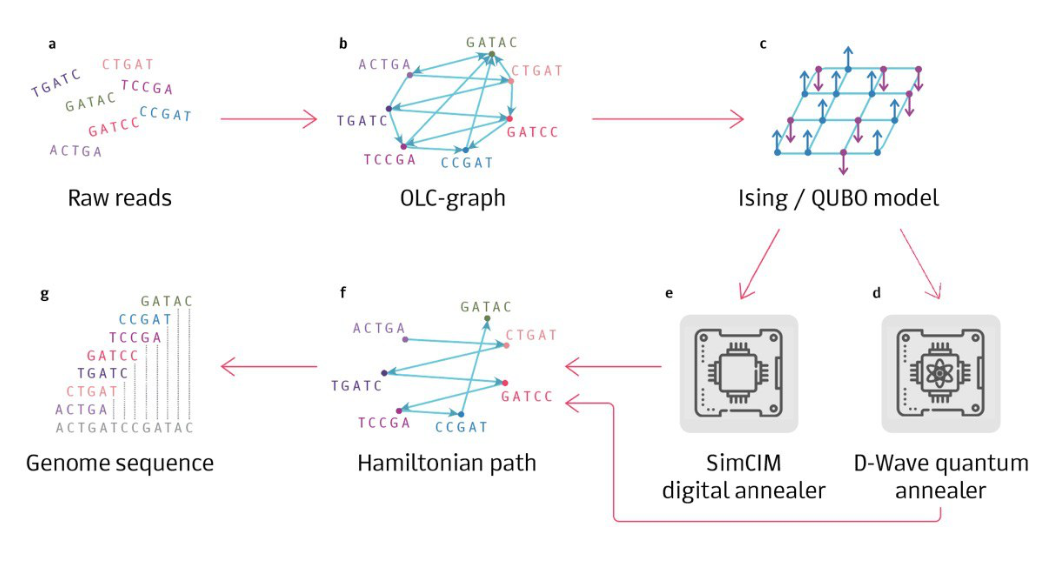
\includegraphics[scale=0.4]{de-novo-process.png}
	\centering
	\caption{Resolution diagram for the genome assembly using quantum annealing \cite{Boev2020}}
	\label{de-novo-process}
\end{figure}


\newparagraph{Numerical example}


Let us study a final numerical example based on \cite{Sarkar2020} that shows the whole process. Suppose we are given the following reads:

\begin{itemize}
	\item $r_0 = ATGGCGTGCA$
	\item $r_1 = GCGTGCAATG$
	\item $r_2 = TGCAATGGCG$
	\item $r_3 = AATGGCGTGC$
\end{itemize}

We may compute the overlap between the different reads. This results in the overlap graph from figure \ref{fig:overlap-graph}.

\begin{figure}[h]
	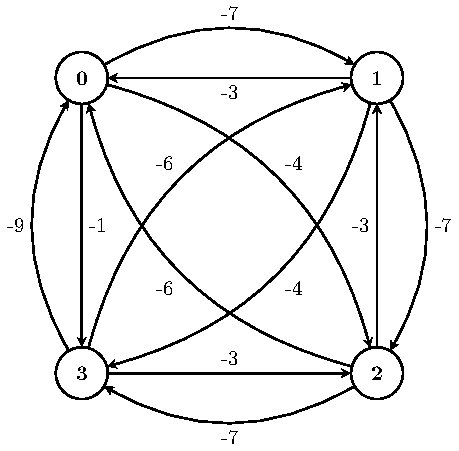
\includegraphics[scale=1.1]{graphs/salesman-example.pdf}
	\centering
	\caption{OLC graph}
	\label{fig:overlap-graph}
\end{figure}

Which is the same graph studied in the traveling salesman section \ref{sec:salesman-example}. From the study done in that section, we know that there are six types of cycles in the graph, as shown in table \ref{tbl:salesman-cycles}. In figure \ref{fig:overlap-cycles}, we see how these type of cycles represent different ordinations of our DNA reads, as well as their overlaps and the total length of the resulting chain.

\begin{figure}[h]
	\makebox[\textwidth][c]{
		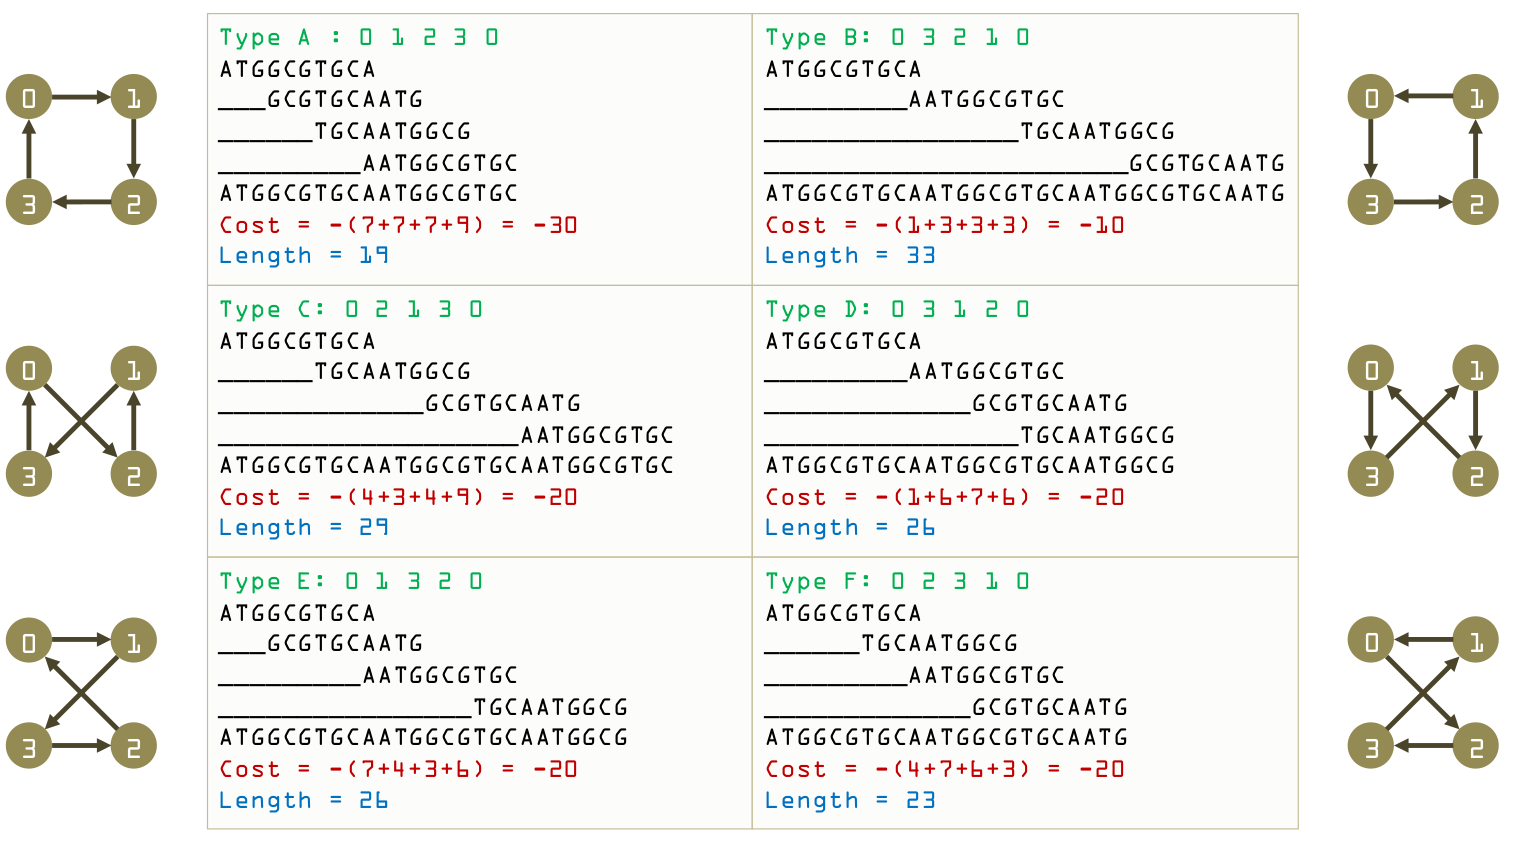
\includegraphics[scale=0.35]{overlap-cycles.png}
	}
	\centering
	\caption{Type of cycles and their corresponding overlap analysis \cite{Sarkar2020}}
	\label{fig:overlap-cycles}
\end{figure}

As we know, the type of Hamiltonian cycle that minimizes the cost is type A. This type translates into the shortest chain, with a total length of $19$. We can easily compute the resulting assembly by traversing the graph and weaving the reads together.


\section{Experimentation}


In this last section, we will explain the experiments reproduced using the D-Wave systems. For this porpouse we used \emph{D-Wave Ocean Software}, a suite of tools provided by D-Wave to use their quantum systems \cite{DWave-OceanDoc}. Using python and the provided packages we may connect to \emph{Leap}, a 'quantum' cloud service that provides access the quantum computers \cite{DWave-Leap}. These experiments are based on \cite{Sarkar2020}.


\subsection{Experiment 1: Data preparation and exact solving}


The first experiment reproduced aims to solve the previously discussed example using the an exact solver provided by the Ocean's \emph{dimod} library \cite{Dimod}. The steps taken to transform the given reads to the QUBO matrix that Ocean's classes and functions use will be shared between the simulated quantum annealer and the real quantum solvers. Therefore, the data preparation applied will be shared between experiments. The pseudocode of the experiment can be seen in the following snippet.

\begin{algorithm}
	\caption*{\textbf{Experiment 1}}
	
	Data preparation:
	\begin{itemize}
		\item Compute the distance between every two reads, creating an adjacency matrix.
		\item Transform the TSP adjancency matrix into a QUBO $Q$ matrix, as explained in section \ref{sec:tsp-qubo}.
		\item Transform the QUBO matrix into an adjacency dictionary.
	\end{itemize}

	Solving:
	\begin{itemize}
		\item Initiaize a sampler: \textbf{\emph{dimod.ExactSolver}}.
		\item Solve the prepared QUBO model using the selected solver.
	\end{itemize}
	
	Print the solutions
\end{algorithm}

As we already know, using quantum annealing does not guarantee that we will obtain the optimal solution for a given cost function. In order to overcome this problem we use multi-sampling: running the experiment multiple times and and look at the best obtained solutions. Ocean already implements different types of \emph{samplers} to facilitate this task \ref{DWave-OceanDoc-Samplers}. In this first experiment we use an \emph{ExactSolver}, which simply check every possible solution. Although time-costly, this method will let us know if our data manipulation before solving the experiment is correct, and how the solutions landscape looks.

The third step in data preparation is a formatting step. Ocean requires the QUBO and Ising models to be in an adjacency dictionary instead of a matrix. Let us look at an example of this transformation in order to better understand it. Consider a 2-reads, the associated TSP will have $2^2 = 4$ nodes: $n0t0$, $n0t1$, $n1t0$ and $n1t1$. Suppose the following (inconsistency) matrix is the associated $Q$ matrix:

$$
Q = 
\left(
\begin{array}{cccc}
	1 & 2 & 0 & -1 \\
	3 & 4 & 0 & 0 \\
	0 & 0 & 0 & 0 \\
	0 & 0 & 100 & 200 
\end{array}
\right)
$$

Then, it will be transformed into the dictionary, with $11$ missing entries: 

\begin{minted}[bgcolor=bg]{python}
quboDict: {
	('n0t0', 'n0t0'): 1,
	('n0t0', 'n0t1'): 2,
	('n0t0', 'n0t2'): 0,
	('n0t0', 'n0t3'): -1,
	...
	('n3t3', 'n3t3'): 200,
}
\end{minted}

In particular, this experiment is applied to the already studied example with the following four reads:

\begin{itemize}
	\item $r_0 = ATGGCGTGCA$
	\item $r_1 = GCGTGCAATG$
	\item $r_2 = TGCAATGGCG$
	\item $r_3 = AATGGCGTGC$
\end{itemize}

The pair-wise distances are computed, providing a direct measure of much two reads overlap. Then, these values are normalized for easier use. This normalized TSP matrix is transformed into a QUBO matrix using $1.6$ as multi-location and repetition penalties, and $-1.6$ for self-bias, as done in \cite{Sarkar2020}. Finally, we initialize a \emph{ExactSolver} and use it to sample every possible solution.

After the execution is completed, we find the lowest energy in the obtained solutions and print every solution with that energy:

\begin{minted}[bgcolor=bg]{python}
{'n0t0': 0, 'n0t1': 0, 'n0t2': 1, 'n0t3': 0,
 'n1t0': 0, 'n1t1': 0, 'n1t2': 0, 'n1t3': 1,
 'n2t0': 1, 'n2t1': 0, 'n2t2': 0, 'n2t3': 0,
 'n3t0': 0, 'n3t1': 1, 'n3t2': 0, 'n3t3': 0} --> -7.9811

{'n0t0': 0, 'n0t1': 1, 'n0t2': 0, 'n0t3': 0,
 'n1t0': 0, 'n1t1': 0, 'n1t2': 1, 'n1t3': 0, 
 'n2t0': 0, 'n2t1': 0, 'n2t2': 0, 'n2t3': 1, 
 'n3t0': 1, 'n3t1': 0, 'n3t2': 0, 'n3t3': 0} --> -7.9811

{'n0t0': 1, 'n0t1': 0, 'n0t2': 0, 'n0t3': 0,
 'n1t0': 0, 'n1t1': 1, 'n1t2': 0, 'n1t3': 0, 
 'n2t0': 0, 'n2t1': 0, 'n2t2': 1, 'n2t3': 0, 
 'n3t0': 0, 'n3t1': 0, 'n3t2': 0, 'n3t3': 1} --> -7.9811

{'n0t0': 0, 'n0t1': 0, 'n0t2': 0, 'n0t3': 1,
 'n1t0': 1, 'n1t1': 0, 'n1t2': 0, 'n1t3': 0,
 'n2t0': 0, 'n2t1': 1, 'n2t2': 0, 'n2t3': 0,
 'n3t0': 0, 'n3t1': 0, 'n3t2': 1, 'n3t3': 0} --> -7.9811
\end{minted}

As expected, these are the four minimums of the cost functions, representing the four ways of describing a type A loop in the used codification.

Finally, let us plot the landscape of solutions for the given reads. We sort the solutions by increasing energy and simply plot their energy, as seen in figure \ref{fig:exp1-landscape}.

\begin{figure}[H]
	\makebox[\textwidth][c]{
		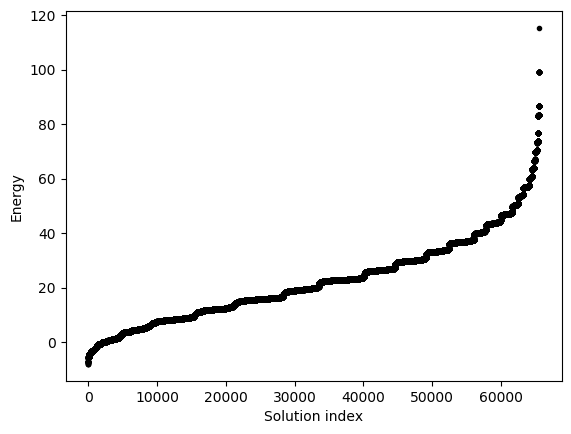
\includegraphics[scale=0.7]{experiments/experiment1.png}
	}
	\centering
	\caption{Landscape of solutions}
	\label{fig:exp1-landscape}
\end{figure}


\subsection{Experiment 2: Simulated Quantum Annealing}


For our second experiment we aim to solve our example using Simulated Annealing. Although \emph{dimod} provides a simulated annealing sampler, we use for our final experiments the  \emph{SimulatedAnnealingSampler} from \emph{Ocean}'s \emph{Neal} package as it yields more distributed results and has far better computing time. The same experiment was reproduced $10$ times using both samplers in my machine. Dimod's sampler obtained a mean time of $11.76$ seconds while \emph{Neal}'s obtained a mean of $0.0610$ seconds.

The pseudo-code doesn change much from the first experiment to the second one, we simply change the annealer:

\begin{algorithm}
	\caption*{\textbf{Experiment 2}}
	
	Data preparation:
	\begin{itemize}
		\item Compute the distance between every two reads, creating an adjacency matrix.
		\item Transform the TSP adjancency matrix into a QUBO $Q$ matrix, as explained in section \ref{sec:tsp-qubo}.
		\item Transform the QUBO matrix into an adjacency dictionary.
	\end{itemize}
	
	Solving:
	\begin{itemize}
		\item Initiaize a sampler: \textbf{\emph{neal.SimulatedAnnealingSampler}}.
		\item \textbf{Sample from} the prepared QUBO model using the selected \textbf{sampler}.
	\end{itemize}
	
	Print the solutions
\end{algorithm}

It is worth mentioning that we don \emph{solve} the QUBO model in this experiment, we \emph{sample} different results using simulated annealing.

Since \emph{Neal}'s sampler is quite efficient we were able to execute experiments with up to $10.000$ repetitions of the experiment, also called \emph{sample reads} or simply \emph{reads}. We developed an automated and escalable way to check whether a given cycle returned by the annealer was valid, and to recover its type. Using this tools we can easily check the number of occurrences each type of cycle appeared in the obtained sample reads. These resulsts are presented, along with the associated energy to each result, in table \ref{tab:exp2} and figure \ref{fig:exp2-occ}. See fig \ref{fig:overlap-cycles} to recall the cycle types and cost computing.

\begin{table}[H]
	\centering
	\begin{tabular}{lrr}
		\textbf{Cycle type} & \textbf{Occurences} & \textbf{Energy} \\
		\hline
		Type A	& 3722	& -7.9811	\\
		Type C	& 1474	& -7.4541	\\
		Type D	& 1469	& -7.4541	\\
		Type F	& 1458	& -7.4541	\\
		Type E	& 1431	& -7.4541	\\
		Type B	& 446	& -6.927                             
	\end{tabular}
	\caption{Results of experiment 2}
	\label{tab:exp2}
\end{table}

\begin{figure}[H]
	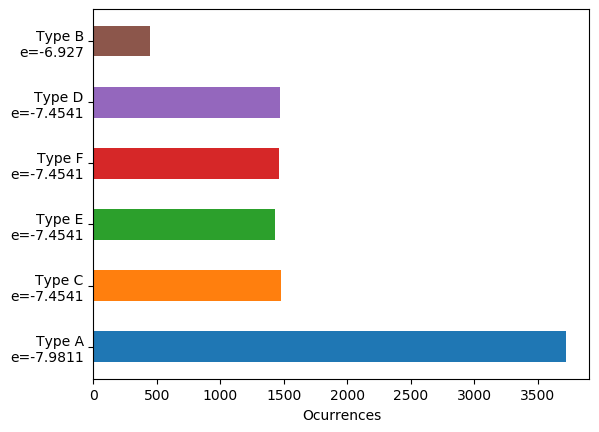
\includegraphics[scale=0.8]{experiments/experiment2.png}
	\centering
	\caption{Ocurrences of each type in a $10.000$ reads experiment using Simulated Annealing}
	\label{fig:exp2-occ}
\end{figure}

We can appreciate in figure \ref{fig:exp2-occ} that best type of cycle agglomerates most of the samples, $37.22\%$. In second place, the four type of cycles that have the exact same energy have each almost exactly the same number of samples. This matches our quantum annealing theory: the phisical system has equal probability of ending in eigen-states with equal eigen-energies.

It is worth mentioning that there was not a single sample that encoded an invalid cycle. This means that the penalties values used for the experiment ($1.6$ for multiĺocation and repetition, and $-1.6$ for self-bias) are well-based.

Now that we are familiar with the type of results and codifications we may find, let us jump to the real Quantum Realm by using the D-Wave's Quantum Computer Systems.


\subsection{Experiment 3: Quantum Annealing using D-Wave}


For our second experiment we aim to solve our example using D-Wave quantum annealers. For this pourpose, we need to add some extra steps to our data processing. Section \ref{sec:embeddings} explained how not every graph can be directly mapped to the existing Chimera / Pegasus topologies that D-Wave systems use, and how we can overcome this problem by embedding our problems graphs into these topologies. The extra steps in our data processing are related to these embeddings: we will need to embed our graph into the fixed topology that will be used, and then translate the solutions from the embedded graph. Ocean provides a set of utilities to deal with embeddings \cite{DWave-OceanDoc-Embedding}.

Additionally, we will need to connect to Leap to send our jobs to the quantum annealers using a \emph{client}. First, a configuration file is created, which includes your API key and some extra configuration details:

\begin{minted}[bgcolor=bg]{bash}
[ocete]
solver = {"qpu": true}
token = DEV-<api key goes here>
endpoint = https://cloud.dwavesys.com/sapi
\end{minted}

In our code we initialize a \emph{client} and a \emph{solver} using the configuration file. These are objects that encapsulate the connection functionality and solving problems in the associated machine respectively. We also initialize a sampler as we did before, but this time a production sampler is used: a \emph{DWaveSampler} that also needs our configuration file. The pseudo-code for this experiment looks as follows. Each new step will be explained in detail below.

\begin{algorithm}
	\caption*{\textbf{Experiment 3}}
	
	Initialization:
	\begin{itemize}
		\item Initiaize a sampler: \textbf{\emph{system.samplers.DWaveSampler}}.
		\item \textbf{Initialize a client and obtain an associated solver}.
	\end{itemize}
	
	Data preparation:
	\begin{itemize}
		\item Compute the distance between every two reads, creating an adjacency matrix.
		\item Transform the TSP adjancency matrix into a QUBO $Q$ matrix, as explained in section \ref{sec:tsp-qubo}.
		\item Transform the QUBO matrix into an adjacency dictionary.
		\item \textbf{Find an embedding from our graph to the used machine topology (either Chimera or Pegasus)}.
		\item \textbf{Use the previous embedding to create a new QUBO model equivalent for the embedded graph}.
	\end{itemize}
	
	Solving:
	\begin{itemize}
		\item Use the solver to send a job to the client. This job samples from the prepared QUBO model multiple times.
	\end{itemize}
	
	Format the results:
	\begin{itemize}
		\item \textbf{Use the computed embedding to translate our answers}.
	\end{itemize}
\end{algorithm}

The first thing to be notice is that the initialization now needs to be done before the data preparation. This is because in order to find the embedding, we need to know which exact topology the quantum system will have. This information is provided through the \emph{solver}, previously initialized. The initialization step is as simple as follows:

\begin{minted}[bgcolor=bg]{python}
import dwave

# Create the solver (connecting to D-Wave) and the Sampler
config_file='../dwave.conf'
client = cloud.Client.from_config(config_file, profile='ocete')
solver = client.get_solver()
dwsampler = system.samplers.DWaveSampler(config_file=config_file)
\end{minted}

Suposse $Q$ already holds are computed QUBO model. We can compute an embedding an obtained the new associated model as follows:

\begin{minted}[bgcolor=bg]{python}
adjacency_dict = embedding.utils.edgelist_to_adjacency(solver.edges)
embedding = minorminer.find_embedding(Q, solver.edges)
Q_embedded = embed_qubo(Q, embedding, adjacency_dict)
\end{minted}

By using the same configuration file, the sampler already knows what machine it is associated to. We will simply sample from it, with the same sintax as in the second experiment:

\begin{minted}[bgcolor=bg]{python}
response = dwsampler.sample_qubo(Q_embedded, num_reads=num_reads)
\end{minted}

Where $num\_reads$ is a parameter that sets the number of samples to be read. However, these solutions are associated to the $Q\_embedded$, not to our original $Q$ model. We need to translate the responses to understand them:

\begin{minted}[bgcolor=bg]{python}
bqm = dimod.BinaryQuadraticModel.from_qubo(Q)
unembedded_response = embedding.unembed_sampleset(response, embedding, bqm)
\end{minted}

For this experiment, the D-Wave 2000Q was used (see section \ref{sec:d-wave-systems} to see its characteristics), since it was the default solver. After running the experiment with the same parameters as the simulated anneling experiment ($10.000$ reads and $(-1.6; 1.6; 1.6)$ for the QUBO parameters), we obtained that more than $90\%$ of the samples were invalid, a huge different with the astonishing $0\%$ obtained in the second experiment.

My initial hypothesis was that the QUBO parameters were well adjusted for SA but not for QA, and thus allowed further tunning. After many attempts with different parameters values, this hypothesis was discarded. The only other set of parameters worth presenting is $(-1.5; 1.5; 1.5)$. These results are presented in table \ref{tab:exp3}.

\begin{table}[H]
	\centering
	\begin{tabular}{lrrr}
		\textbf{Cycle type} & \textbf{Occurences (1.5)} & \textbf{Occurences (1.6)} & \textbf{Energy} \\
		\hline
		Type A	& 131	& 50	& -7.9811	\\
		Type C	& 124	& 46	& -7.4541	\\
		Type D	& 40	& 91	& -7.4541	\\
		Type F	& 55	& 117	& -7.4541	\\
		Type E	& 112	& 118	& -7.4541	\\
		Type B	& 99	& 64	& -7.4541	\\    
		Invalid & 9221	& 9194	& $>$ -5.6433                         
	\end{tabular}
	\caption{Results of experiment 3}
	\label{tab:exp3}
\end{table}

In figures \ref{fig:exp3-occ1} and \ref{fig:exp3-occ2} we see a comparisson of the distribution between the different type of cycles in both experiments. We cannot see a distribution as we did in \ref{fig:exp2-occ}, potentially due to the low numbers of reads that actually represent a valid cycle. We do know that we are not sampling completely random solutions: in a 4-reads problems with obtain a 16 variables QUBO model, with up to $2^16$ possible solutions using our encoding. That is, previous embedding the graph in the topology.

In fact, such distribution between the cycle types is not needed: a single sample with the lowest energy solution will completely solve our genome assembly problem.

\begin{figure}[H]
	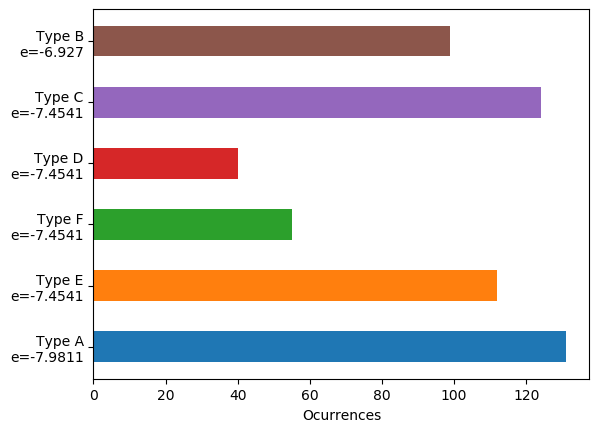
\includegraphics[scale=0.75]{experiments/experiment3 (1.5).png}
	\centering
	\caption{Ocurrences of each cycle type in a $10.000$ reads experiment using Quantum Annealing, filtering out invalid cycles, with QUBO parameters $(-1.5; 1.5; 1.5)$}
	\label{fig:exp3-occ1}
\end{figure}

\begin{figure}[H]
	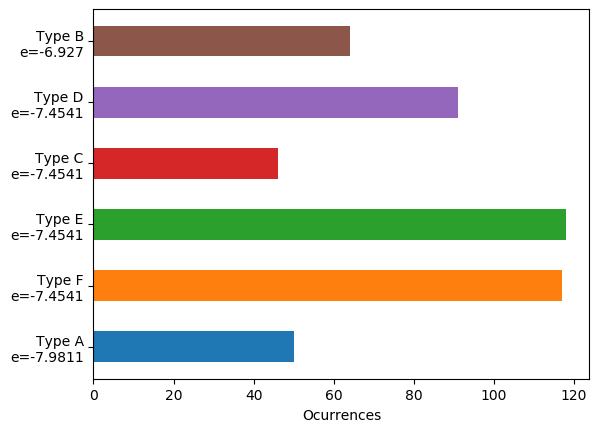
\includegraphics[scale=0.75]{experiments/experiment3 (1.6).png}
	\centering
	\caption{Ocurrences of each cycle type in a $10.000$ reads experiment using Quantum Annealing, filtering out invalid cycles, with QUBO parameters $(-1.6; 1.6; 1.6)$}
	\label{fig:exp3-occ2}
\end{figure}

Therefore, we have not find a clear improvement precision-wise in our small example, although QA solves the problem. What about time-wise? In figure \ref{fig:exp3-time} we see the time breakdown provided by Ocean after our last experiment. We can see a total QPU sampling time of $2.389$ seconds, while if we repeat the experiment with the same parameters using SA we obtain a mean of $2.525$ sampling seconds, over $10$ experiment repetitions. Keeping in mind that our QA time data comes from a single execution and the small difference between both time measures, we cannot conclude that either approach has any time advantage in such small problems.

However, does QA actually scales better than SA with the problem size? In the next experiment we will study the Pegasus topology to understand what is the maximum problem size that can be tackled using the Advantage system. Finally, the last experiment will try to answer the scalability comparison inquiry.

\begin{figure}[h]
	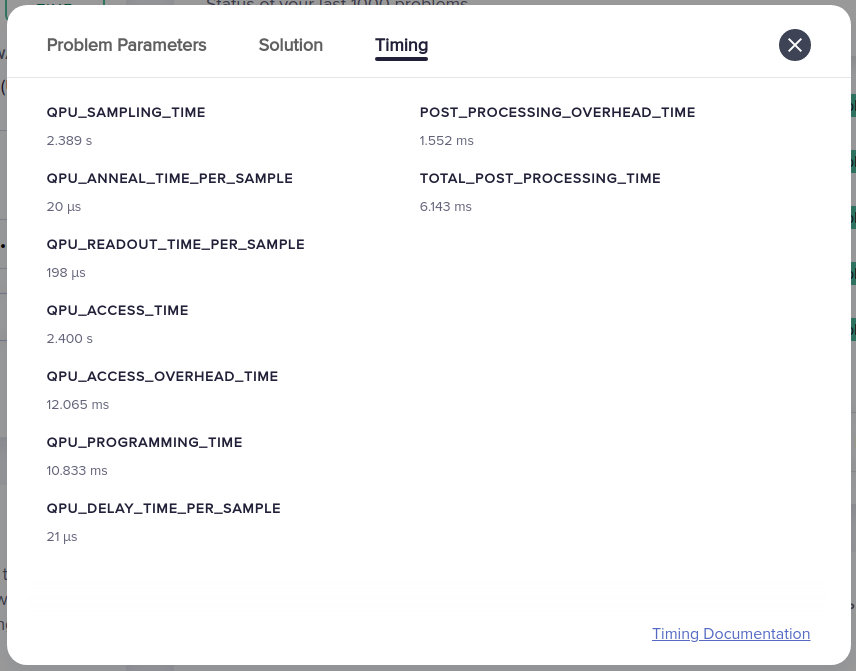
\includegraphics[scale=0.5]{experiments/exp3-time.png}
	\centering
	\caption{Time breakdown provided by Ocean after the last experiment.}
	\label{fig:exp3-time}
\end{figure}


\subsection{Experiment 4: D-Wave's Advantage limits}

\subsection{Experiment 5: Scalability comparison between Simulated Annealing and Quantum Annealing}


